\documentclass[11pt]{article}
\usepackage[margin=1in]{geometry}
\usepackage{amsmath,amssymb,bm}
\usepackage{booktabs}
\usepackage{xcolor}
\usepackage{listings}
\usepackage{tikz}
\usetikzlibrary{shapes.geometric,arrows.meta,positioning}
\usepackage{hyperref}
\hypersetup{colorlinks=true,linkcolor=blue,urlcolor=blue}

\definecolor{codebg}{rgb}{0.96,0.96,0.94}
\definecolor{kw}{rgb}{0.0,0.0,0.6}
\definecolor{cm}{rgb}{0.30,0.45,0.30}
\definecolor{st}{rgb}{0.6,0.1,0.1}
\lstset{
  basicstyle=\ttfamily\footnotesize,
  backgroundcolor=\color{codebg},
  keywordstyle=\color{kw}\bfseries,
  commentstyle=\color{cm}\itshape,
  stringstyle=\color{st},
  language=Python,
  showstringspaces=false,
  breaklines=true,
  frame=single,
  columns=fullflexible,
  morekeywords={self,np}
}

\newcommand{\cre}[1]{\hat{c}^{\dagger}_{#1}}
\newcommand{\ann}[1]{\hat{c}^{\phantom{\dagger}}_{#1}}
\newcommand{\bs}[1]{\boldsymbol{#1}}
\newcommand{\ket}[1]{\left|#1\right\rangle}
\newcommand{\bra}[1]{\left\langle#1\right|}
\newcommand{\bracket}[2]{\left\langle#1\middle|#2\right\rangle}
\newcommand{\dt}{\Delta\tau}
\newcommand{\psiT}{\ket{\psi_T}}

\title{\textbf{Constrained-Path Auxiliary-Field Quantum Monte Carlo}\\[2pt]
\large Theory, Algorithm, and the \texttt{pyqmc} Implementation}
\author{CPQMC validation platform --- \texttt{codex\_CPQMC/pyqmc}}
\date{\today}

\begin{document}
\maketitle

\begin{abstract}
This note derives the constrained-path auxiliary-field quantum Monte Carlo
(CP-AFQMC / CPMC) algorithm of Zhang and Krakauer as implemented in
\texttt{pyqmc/cpqmc.py}, the Python port of the validation platform. We give the
ground-state projection, the Trotter--Suzuki split, the discrete
Hubbard--Stratonovich transformation actually used in the code, importance
sampling, the constrained-path approximation, the mixed and back-propagated
estimators, and the observables (energy, equal-time correlations, singlet pairing,
magnetization). We close with the adaptive self-consistent trial wavefunction
(Phase~6), an algorithm flowchart, and a line-by-line map from the equations to
the code.
\end{abstract}

\tableofcontents

\section{Model}
The platform targets density--density lattice fermion Hamiltonians,
\begin{equation}
\hat H = \hat K + \hat V,\qquad
\hat K = \sum_{ij,\sigma} K_{ij}\,\cre{i\sigma}\ann{j\sigma},\qquad
\hat V = \sum_{(a s_a,\, b s_b)} V_{ab}\, \hat n_{a s_a}\hat n_{b s_b},
\label{eq:H}
\end{equation}
with $\hat n_{a\sigma}=\cre{a\sigma}\ann{a\sigma}$. The single-band Hubbard model
has $K_{ij}=-t$ on nearest neighbours and a single on-site term
$V=U$, $\hat V = U\sum_i \hat n_{i\uparrow}\hat n_{i\downarrow}$. The two-orbital
altermagnet (the PRL LE20050 model) uses the anisotropic two-orbital hopping
$K$ built in \texttt{altermagnet\_ed.build\_hopping}, plus on-site $u_{xx}$,
inter-orbital $u_{xy}$, and neighbour $v$ (intra-orbital $+v$, inter-orbital
$-v$). All three reduce to the general density--density form of
Eq.~\eqref{eq:H}, which is why a single propagation/estimator engine covers
every channel.

\begin{lstlisting}[caption={Interaction stored as a generic density--density term
list (\texttt{LatticeModel.\_build\_terms}).}]
# on-site Hubbard U on every (orbital-)site: n_{i,up} n_{i,dn}
self.terms.append((i, 0, i, 1, e1, e2, cf))     # (a, s_a, b, s_b, HS factors)
self.pot_terms.append((i, 0, i, 1, U))          # (a, s_a, b, s_b, V)
\end{lstlisting}

\section{Ground-state projection}
CPMC obtains the ground state by imaginary-time projection from a trial state
$\psiT$ non-orthogonal to it,
\begin{equation}
\ket{\psi_0}\ \propto\ \lim_{\beta\to\infty} e^{-\beta \hat H}\psiT
= \lim_{n\to\infty}\left(e^{-\dt \hat H}\right)^{n}\psiT,
\qquad \beta = n\,\dt .
\label{eq:proj}
\end{equation}
The trial is taken as the free-electron ground state of $\hat K$ (the lowest
$N_\uparrow$ / $N_\downarrow$ eigenvectors), a single Slater determinant per spin.

\begin{lstlisting}[caption={Trial = free-electron ground state
(\texttt{CPMC.\_\_init\_\_}).}]
w, vecs = np.linalg.eigh(self.K)            # single-particle eigenstates
self.trial = TrialWF(vecs[:, :nup].copy(), vecs[:, :ndn].copy())
\end{lstlisting}

\section{Trotter--Suzuki decomposition}
For small $\dt$ the symmetric (second-order) split separates kinetic and
interaction parts,
\begin{equation}
e^{-\dt \hat H} = e^{-\frac{\dt}{2}\hat K}\, e^{-\dt \hat V}\,
e^{-\frac{\dt}{2}\hat K} + \mathcal{O}(\dt^{3}).
\label{eq:trotter}
\end{equation}
The one-body factor $B_K \equiv e^{-\frac{\dt}{2}\hat K}$ acts on a Slater
determinant $\Phi$ (an $N_s\times N_\sigma$ matrix of orbitals) by left
multiplication, $\Phi\to e^{-\frac{\dt}{2}K}\Phi$, preserving the determinant
form (Thouless' theorem).

\begin{lstlisting}[caption={Half-step kinetic propagator
(\texttt{LatticeModel}).}]
self.expK = vecs @ np.diag(np.exp(-0.5 * dt * w)) @ vecs.T   # e^{-dt K/2}
\end{lstlisting}

\section{Discrete Hubbard--Stratonovich transformation}
The interaction $e^{-\dt V \hat n_a \hat n_b}$ is quartic in the fermion
operators; it is decoupled into a sum over an Ising-like auxiliary field
$s=\pm1$ so that each term becomes a one-body operator. For each density--density
pair the code uses the discrete Hirsch decoupling. Writing
$\cosh\gamma = e^{\frac{\dt}{2}|V|}$:
\begin{itemize}
\item \textbf{Repulsive} ($V>0$): the \emph{spin} channel,
\begin{equation}
e^{-\dt V \hat n_a\hat n_b}
= e^{-\frac{\dt V}{2}(\hat n_a+\hat n_b)}\,
\tfrac12\!\!\sum_{s=\pm1} e^{\gamma s(\hat n_a-\hat n_b)} ,
\label{eq:hsrep}
\end{equation}
implemented as operator-1 on $(a,s_a)$ with factor $e^{\gamma s-\dt V/2}$ and
operator-2 on $(b,s_b)$ with factor $e^{-\gamma s-\dt V/2}$.
\item \textbf{Attractive} ($V<0$): the \emph{charge} channel; both operators take
$e^{\gamma s-\dt V/2}$ and the field carries a weight $e^{-\gamma s+\dt V/2}$.
\end{itemize}
For the on-site Hubbard term $a=b=i$, $s_a=\uparrow$, $s_b=\downarrow$,
Eq.~\eqref{eq:hsrep} is the textbook Hirsch transform with
$\cosh\gamma=e^{\dt U/2}$.

\begin{lstlisting}[caption={Discrete HS factors (\texttt{LatticeModel.\_hs}).}]
a = np.arccosh(np.exp(0.5 * dt * abs(V)))            # gamma, cosh(g)=e^{dt|V|/2}
if V > 0:                                            # repulsive: spin channel
    e1 = np.array([np.exp(a - 0.5*dt*V), np.exp(-a - 0.5*dt*V)])
    e2 = np.array([np.exp(-a - 0.5*dt*V), np.exp(a - 0.5*dt*V)])
    cf = np.array([1.0, 1.0])
else:                                                # attractive: charge channel
    e1 = np.array([np.exp(a - 0.5*dt*V), np.exp(-a - 0.5*dt*V)]); e2 = e1.copy()
    cf = np.array([np.exp(-a + 0.5*dt*V), np.exp(a + 0.5*dt*V)])
\end{lstlisting}

After the transformation a full time step is a \emph{sum over auxiliary-field
configurations} of one-body propagators:
\begin{equation}
e^{-\dt \hat H}\,\Phi
= \sum_{\{s\}} P(\{s\})\; B_K\, B_V(\{s\})\, B_K\,\Phi,
\label{eq:walk}
\end{equation}
each $B_V(\{s\})$ being diagonal scalings of the determinant rows. Because a
one-body operator maps a Slater determinant to a Slater determinant, the
projection \eqref{eq:proj} becomes an open-ended random walk in the manifold of
determinants.

\section{Random walk, importance sampling, constrained path}
A population of \emph{walkers} $\{\ket{\phi_i}, w_i\}$ represents the projected
state stochastically, $\ket{\psi}\approx\sum_i w_i \ket{\phi_i}/\bracket{\psi_T}{\phi_i}$.
Naive sampling of $\{s\}$ has a large variance; the code uses
\emph{importance sampling}, choosing each field with probability proportional to
the overlap ratio with the trial,
\begin{equation}
p_s \propto c_s \,\max\!\left(
\frac{\bracket{\psi_T}{\phi^{(s)}}}{\bracket{\psi_T}{\phi}},\,0\right),
\label{eq:imp}
\end{equation}
where $\phi^{(s)}$ is the determinant after applying the field-$s$ one-body
factor and $c_s$ is the HS weight ($\texttt{cf}$). The walker weight is multiplied
by the normalization $w_i \to w_i\cdot\tfrac12\sum_s c_s R_s$.

\paragraph{Constrained-path approximation.}
The $\max(\cdot,0)$ in Eq.~\eqref{eq:imp} is the constrained path: walkers whose
overlap with the trial would turn non-positive are removed. This eliminates the
fermion sign problem (the walk stays in the half-space
$\bracket{\psi_T}{\phi}>0$) at the cost of a bias that vanishes as $\psiT\to\psi_0$.

\begin{lstlisting}[caption={One importance-sampled, constrained step
(\texttt{Propagator.step}).}]
for (a, sa, b, sb, e1, e2, cf) in m.terms:
    ratios = np.empty(2)
    for k in (0, 1):                       # HS field s = +1 (k=0), -1 (k=1)
        R = self._term_ratio(pu, pd, ov_up, ov_dn, a, sa, b, sb, e1[k], e2[k])
        ratios[k] = cf[k] * max(R, 0.0)    # constrained path: clip R <= 0
    tot = ratios.sum()
    if tot <= 0:
        walkers.w[i] = 0.0; killed = True; break
    k = self.rng.choice(2, p=ratios / tot)    # importance sampling
    # ... apply chosen one-body factor to rows a, b ...
    walkers.w[i] *= 0.5 * tot
\end{lstlisting}

\paragraph{Stabilization and population control.}
Repeated $B_K$ multiplication makes the orbital columns numerically collinear;
the code periodically re-orthonormalizes each determinant by a QR factorization
(the determinant is invariant up to the discarded $R$). A comb-resampling
population-control step keeps the walker count fixed while pruning small weights
and branching large ones.

\section{Estimators}
\subsection{Mixed estimator}
For an operator $\hat O$ the mixed estimator is
\begin{equation}
\langle \hat O\rangle_{\rm mix}
= \frac{\sum_i w_i\, \dfrac{\bra{\psi_T}\hat O\ket{\phi_i}}{\bracket{\psi_T}{\phi_i}}}
       {\sum_i w_i}.
\label{eq:mixed}
\end{equation}
Matrix elements between Slater determinants reduce, by the generalized Wick
theorem, to the single-particle Green's function
\begin{equation}
G^{\sigma}_{ij}
= \frac{\bra{\psi_T}\cre{i\sigma}\ann{j\sigma}\ket{\phi}}{\bracket{\psi_T}{\phi}}
= \left[\Phi\,(\Psi_T^{\dagger}\Phi)^{-1}\Psi_T^{\dagger}\right]_{ji}.
\label{eq:green}
\end{equation}
The energy is exact for $\hat H$ (zero-variance principle) at $\psiT=\psi_0$;
operators not commuting with $\hat H$ carry an $O(\text{systematic})$ bias.

\begin{lstlisting}[caption={Green's function and mixed energy
(\texttt{Estimators.energy}).}]
def _green(left, phi):
    A = left.T @ phi
    return phi @ np.linalg.solve(A, left.T)   # G_ij = <c^+_j c_i>
...
ek = np.sum(m.K * Gu.T) + np.sum(m.K * Gd.T)  # kinetic
ev += V * (Gs[a,a]*Gs[b,b] - Gs[a,b]*Gs[b,a]) # same-spin Wick (exchange)
ev += V *  G[sa][a,a]*G[sb][b,b]              # opposite-spin (no exchange)
\end{lstlisting}

\subsection{Back-propagation}
The mixed bias for $\hat O\neq f(\hat H)$ is removed by back-propagation: the bra
$\psiT$ is itself projected for $m$ steps using the \emph{recorded} auxiliary
fields, $\bra{\psi_T}\to\bra{\psi_T}\prod B^{\dagger}$, giving a pure (left/right
both projected) estimator
\begin{equation}
\langle\hat O\rangle_{\rm bp}
= \frac{\sum_i w_i\,
\bra{\psi_T}\!\Big(\textstyle\prod_l B_l\Big)^{\!\dagger}\hat O\ket{\phi_i}}
{\sum_i w_i\,\bra{\psi_T}\!\big(\prod_l B_l\big)^{\!\dagger}\ket{\phi_i}} .
\label{eq:bp}
\end{equation}
The constrained-path bias from the trial \emph{node} remains; back-propagation
removes only the mixed-estimator part.

\begin{lstlisting}[caption={Back-propagated bra (\texttt{Estimators.bp\_bra}).}]
Lu = tr.up.copy(); Ld = tr.dn.copy()
for s in range(bp - 1, -1, -1):               # replay recorded fields, reversed
    Lu = m.expK @ Lu; Ld = m.expK @ Ld
    for (a, sa, b, sb, e1, e2, cf), k in zip(m.terms, ch):
        # apply the recorded field-k factors to the bra
    Lu = m.expK @ Lu; Ld = m.expK @ Ld
\end{lstlisting}

\subsection{Two-body observables}
Equal-time correlations follow from $G$ by Wick's theorem (spin-separated
determinants, so no cross-spin contraction):
\begin{align}
\langle \hat n_i \hat n_j\rangle &=
(n^{\uparrow}_i+n^{\downarrow}_i)(n^{\uparrow}_j+n^{\downarrow}_j)
+\!\!\sum_{\sigma}\!\big(\delta_{ij}n^{\sigma}_i - G^{\sigma}_{ij}G^{\sigma}_{ji}\big),\\
\langle S^z_i S^z_j\rangle &= \tfrac14\Big[
(n^{\uparrow}_i-n^{\downarrow}_i)(n^{\uparrow}_j-n^{\downarrow}_j)
+\!\!\sum_{\sigma}\!\big(\delta_{ij}n^{\sigma}_i - G^{\sigma}_{ij}G^{\sigma}_{ji}\big)\Big].
\end{align}
The singlet pairing structure factor for symmetry $\alpha$ with bond form factor
$f_\alpha$ and pair operator
$\hat\Delta_\alpha(m)=\sum_{\delta}f_\alpha(\delta)\,\ann{m\uparrow}\ann{m+\delta\,\downarrow}$
is
\begin{equation}
S_\alpha=\sum_{m,n}\langle\hat\Delta^{\dagger}_\alpha(m)\hat\Delta_\alpha(n)\rangle
=\sum_{m,n} G^{\uparrow}_{mn}\,\big(B_\alpha G^{\downarrow}B_\alpha^{\!\top}\big)_{mn},
\quad (B_\alpha)_{m,\,m+\delta}=f_\alpha(\delta),
\label{eq:pair}
\end{equation}
exact at $U=0$ and used for the $s$- and $d_{x^2-y^2}$-wave channels
(\texttt{Estimators.pairmag\_block}).

\subsection{Dynamic (imaginary-time-displaced) correlations}
Unequal-time correlations $C_O(\tau)=\bra{\psi_0}\hat O\,e^{-\tau(\hat H-E_0)}\hat O
\ket{\psi_0}$ and the static susceptibility $\chi_O=\int_0^\infty\!C_O(\tau)\,d\tau$
follow from the imaginary-time-displaced single-particle Green's functions. With
the one-body slice propagator $B_{(\ell)}=B_\ell\cdots B_1$ (built from the recorded
auxiliary fields), and $g^\sigma_{ij}=\langle\cre{i\sigma}\ann{j\sigma}\rangle$ the
back-propagated equal-time function, the particle and hole displaced functions and
the displaced density are
\begin{equation}
P^\sigma(\tau)=B_{(\ell)}(I-g^{\sigma\top}),\quad
H^\sigma(\tau)=B_{(\ell)}^{-\top} g^\sigma,\quad
g^\sigma(\tau)=B_{(\ell)}^{-\top} g^\sigma B_{(\ell)}^{\top},
\label{eq:disp}
\end{equation}
using $\ann{i}(\tau)=\sum_j[B_{(\ell)}]_{ij}\ann{j}$ and
$\cre{i}(\tau)=\sum_k[B_{(\ell)}^{-\top}]_{ik}\cre{k}$. The same-spin
density--density correlation is then
$\langle \hat n_{i\sigma}(\tau)\hat n_{j\sigma}(0)\rangle_c
= H^\sigma_{ij}(\tau)\,P^\sigma_{ij}(\tau)$, from which the staggered spin
correlation $C(\tau)=\sum_{ij}(-1)^{r_i+r_j}\langle S^z_i(\tau)S^z_j(0)\rangle$ is
assembled. (The transposes in Eq.~\eqref{eq:disp} are invisible at $U=0$, where
$B$ and $g$ are symmetric, but essential once interacting --- the code is
validated against the ED Lehmann representation
$C(\tau)=\sum_n|\bra{n}\hat O\ket{\psi_0}|^2 e^{-(E_n-E_0)\tau}$.)

\begin{lstlisting}[caption={Time-displaced GFs (\texttt{Estimators.chi\_block}).}]
nu = np.diag(Bui.T @ gu @ Bu.T)               # density n^up_i(tau)
Hu = Bui.T @ gu;  Pu = Bu @ ImguT             # hole / particle displaced GF
conn = 0.25*(phase @ (Hu*Pu) @ phase + phase @ (Hd*Pd) @ phase)  # same-spin
\end{lstlisting}

\section{Adaptive self-consistent trial (Phase 6)}
Because the constrained-path bias is controlled entirely by the quality of
$\psiT$, the code can replace the fixed free-electron trial by a
self-consistent one. Each generation it forms the weighted ensemble one-body
density matrix, symmetrizes it, damps it toward the current trial projector, and
takes the highest-occupation natural orbitals as the new trial:
\begin{equation}
\rho^{\sigma} = \frac{\sum_i w_i G^{\sigma}_i}{\sum_i w_i},\quad
\tilde\rho^{\sigma}= \mu\,\Psi_T^{\sigma}\Psi_T^{\sigma\top}
+(1-\mu)\,\tfrac12(\rho^{\sigma}+\rho^{\sigma\top}),\quad
\Psi_T^{\sigma}\leftarrow \text{top-}N_\sigma\ \text{eigvecs}(\tilde\rho^{\sigma}).
\label{eq:adapt}
\end{equation}
This moves the constraint boundary toward the true ground state. It is
\emph{non-variational} (the trial is no longer a fixed external constraint), so
its benefit is assessed empirically against ED; \texttt{fixed} remains the
validated default.

\begin{lstlisting}[caption={Natural-orbital self-consistent update
(\texttt{TrialWF.update}).}]
ru += w * Gu; rd += w * Gd; W += w            # ensemble 1-RDM
ru = 0.5*(ru+ru.T); rd = 0.5*(rd+rd.T)        # symmetrize (mixed RDM not Herm.)
ru = self.mix*Pu + (1-self.mix)*ru            # damp toward current trial
_, Vu = np.linalg.eigh(ru); self.up = Vu[:, -self.nup:].copy()   # natural orbitals
\end{lstlisting}

\section{Algorithm}
\begin{center}
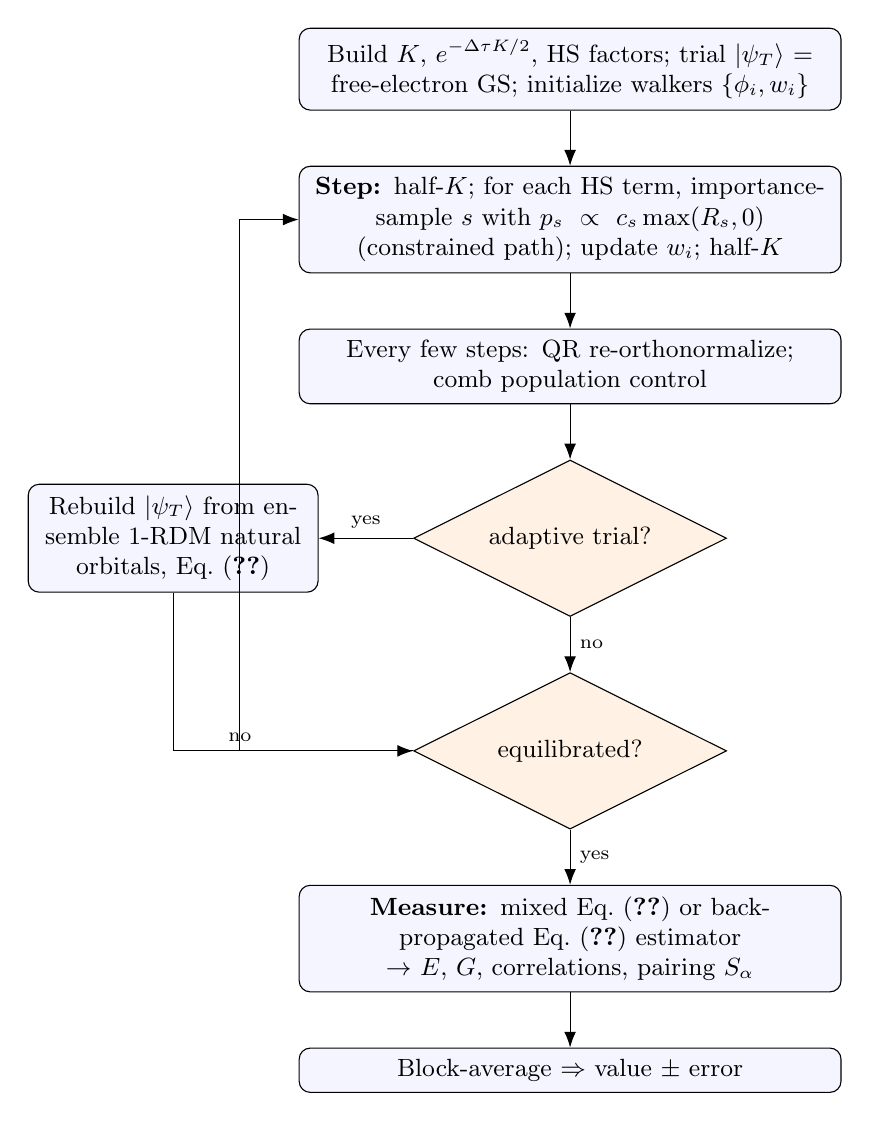
\begin{tikzpicture}[
  node distance=7mm and 12mm,
  box/.style={rectangle,draw,rounded corners,align=center,fill=blue!4,
    inner sep=4pt,font=\small,text width=6.6cm},
  dec/.style={diamond,draw,aspect=2,align=center,fill=orange!10,
    inner sep=1pt,font=\small,text width=3.2cm},
  arr/.style={-{Latex[length=2mm]}}, every node/.style={}]
  \node[box] (init) {Build $K$, $e^{-\dt K/2}$, HS factors; trial $\psiT$
    $=$ free-electron GS; initialize walkers $\{\phi_i,w_i\}$};
  \node[box,below=of init] (step) {\textbf{Step:} half-$K$; for each HS term,
    importance-sample $s$ with $p_s\propto c_s\max(R_s,0)$ (constrained path);
    update $w_i$; half-$K$};
  \node[box,below=of step] (stab) {Every few steps: QR re-orthonormalize;
    comb population control};
  \node[dec,below=of stab] (adapt) {adaptive trial?};
  \node[box,left=of adapt,text width=3.4cm] (upd) {Rebuild $\psiT$ from
    ensemble 1-RDM natural orbitals, Eq.~(\ref{eq:adapt})};
  \node[dec,below=of adapt] (eq) {equilibrated?};
  \node[box,below=of eq] (meas) {\textbf{Measure:} mixed Eq.~(\ref{eq:mixed}) or
    back-propagated Eq.~(\ref{eq:bp}) estimator $\to$ $E$, $G$, correlations,
    pairing $S_\alpha$};
  \node[box,below=of meas] (avg) {Block-average $\Rightarrow$ value $\pm$ error};
  \draw[arr] (init) -- (step);
  \draw[arr] (step) -- (stab);
  \draw[arr] (stab) -- (adapt);
  \draw[arr] (adapt) -- node[above,font=\scriptsize]{yes} (upd);
  \draw[arr] (upd) |- (eq);
  \draw[arr] (adapt) -- node[right,font=\scriptsize]{no} (eq);
  \draw[arr] (eq.west) -- ++(-2.2,0) node[above,font=\scriptsize]{no} |- (step.west);
  \draw[arr] (eq) -- node[right,font=\scriptsize]{yes} (meas);
  \draw[arr] (meas) -- (avg);
\end{tikzpicture}
\end{center}

\section{Theory $\leftrightarrow$ code map}
\begin{center}
\begin{tabular}{lll}
\toprule
Concept & Equation & Code (\texttt{pyqmc/cpqmc.py})\\
\midrule
Model / interaction list & \eqref{eq:H} & \texttt{LatticeModel.\_build\_terms}\\
Half-step kinetic $B_K$ & \eqref{eq:trotter} & \texttt{LatticeModel.expK}\\
Discrete HS factors & \eqref{eq:hsrep} & \texttt{LatticeModel.\_hs}\\
Importance + constraint & \eqref{eq:imp} & \texttt{Propagator.step}\\
Field recording (for BP) & \eqref{eq:bp} & \texttt{Propagator.step\_record}\\
QR stabilize / pop control & --- & \texttt{WalkerEnsemble.reorthogonalize/pop\_control}\\
Green's function & \eqref{eq:green} & \texttt{\_green}\\
Mixed energy & \eqref{eq:mixed} & \texttt{Estimators.energy}\\
Back-propagated bra & \eqref{eq:bp} & \texttt{Estimators.bp\_bra,\ energy\_bp}\\
Pairing / magnetization & \eqref{eq:pair} & \texttt{Estimators.pairmag\_block}\\
Dynamic susceptibility & \eqref{eq:disp} & \texttt{Estimators.chi\_block,\ run\_bp\_chi}\\
Adaptive trial & \eqref{eq:adapt} & \texttt{TrialWF.update}\\
\bottomrule
\end{tabular}
\end{center}

\paragraph{Validation status.} Energy agrees with ED on all three interaction
channels ($u_{xx},u_{xy},v$); equal-time correlations and the pairing/spin
estimators are exact at $U=0$ and carry the expected constrained-path bias when
interacting; the adaptive trial reduces that bias toward ED. See
\texttt{docs/VALIDATION.md} for the quantitative log.

\end{document}
